The Gravitational Search Algorithm (GSA) \cite{GSA} was introduced in 2009, developed as another option for non-linear optimisation.
Where the majority of nature-based optimisation algorithms use multiple agents with some form of swarm intelligence to perform exploration of the search space and exploitation of found maximums, GSA uses multiple agents but with rules based on Newtonian gravity and motion.

In GSA, Gravitational forces are applied on and between agents in the search space, with the mass of an agent is based on its fitness compared to the other agents (a more fit agent is more massive).
Agents are initially randomly distributed throughout the search space.
The new velocity (and hence position) of an agent at each time step is calculated by randomly retaining a portion of the previous velocity, and applying any acceleration due to gravity.
The force due to gravity and the total number of agents can be modified over time steps, for example to have lower initial gravity to promote early exploration, or to reduce the number of agents later on to simplify the system and promote exploitation.
% While Newtonian gravity has masses attracted inversely proportional to the square of their distance (with $F \propto \frac{1}{R^2}$), the original paper on GSA has the force inversely proportional to their distance ($F \propto \frac{1}{R}$).
% Different implementations and versions of the GSA algorithm use either $R$ or $R^2$ - for example of the two papers discussed below, GGSA uses $R$, and EGSA uses $R^2$.


\subsection{Motivation for improvements to GSA}\label{sec:alg:gsa:motiviation}
While GSA performed better in accuracy and convergence speed on benchmarks than other popular algorithms of the time such as PSO and Real Genetic Algorithm \cite{GSA}, there are a number of issues that have lead to modified versions of GSA being proposed and utilised.

The two phases of these nature-inspired algorithms - exploration and exploitation - generally conflict, with increasing the performance of an algorithm in one phase generally weakening the performance in the other.
To combat this, hybrid algorithms combining multiple optimisation algorithms have been tested, for example SA-PSO (see Section \ref{sec:sec:alg:sa-pso} of this report) that uses Simulated Annealing to improve the exploitation performance of the PSO algorithm.
However, while combining multiple algorithms this way improves performance, it can come at the cost of considerable additional computation, potentially even greater than the sum of running each algorithm sequentially.
GSA is an effective optimisation algorithm for large-scale problems, as it is able to perform effectively with a significantly smaller agent count than other algorithms such as PSO \cite{EGSA}, however it is not exempt from the trade-off of exploration vs exploitation.
Local search has been suggested as a way to improve its exploitation \cite{GSA}, but is also computationally expensive particularly in higher dimensional search spaces.
Thus, improvements able to be made to the exploration and exploitation performance of algorithms with minimal additional computational power would be of interest for large-scale problems where it might be infeasible to use hybrid algorithms or local search.


\subsection{Enhanced GSA}\label{sec:alg:gsa:egsa}
Optimal Power Flow (OPF) for electrical grids is a large-scale optimisation problem of obvious interest to reduce operational costs, network losses, and environmental pollution.
It has a discontinuous, nonlinear, and very large solution space making it difficult or infeasible to utilise some optimisation algorithms.
Enhanced GSA (EGSA) was proposed by Jahan and Amjady \cite{EGSA} in 2013 to improve on the exploration of GSA, particularly for a problem with such a large solution space.
The key modification in EGSA is the introduction of a 'mutation' operator, which continuously generates new agents throughout the solution space.
When a mutation is performed, up to half of the worst agents are randomly selected, and a random number of their variables (position within a particular dimension) are changed to random values.
Initially the random values can be from anywhere in that dimension to assist with exploring the entire solution space early on, with the size of the possible change being restricted and reduced as the number of iterations increase to support convergence later on in the search.

To evaluate the proposed algorithm, the paper selected a number of standard OPF optimisation algorithms (Genetic Algorithm, Differential Evolution, PSO, and GSA).
Each algorithm, along with EGSA, were then benchmarked using 5 sample problems - 4 standard but small OPF IEEE datasets, and an additional less standard but significantly larger dataset.
Each algorithm was given 100 agents and 1000 iterations.
While GSA consistently performed well, EGSA outperformed all other algorithms on all sample problems - both with more optimal results, and requiring less compute time.
Additionally, EGSA was the only algorithm that found a solution for the large dataset that was actually economically viable to utilise.
While these results do demonstrate that EGSA (and GSA) is a more effective optimisation algorithm for this type of problem (very large and discontinuous search space, with solution evaluation being expensive) than other optimisation algorithms, it doesn't necessarily extend to simpler or smaller scale problems where the advantages of other algorithms may more heavily outweigh the advantages EGSA has in computational efficiency.


\subsection{Gbest-guided GSA}\label{sec:alg:gsa:ggsa}
As the number of iterations of GSA increase agents all increase in mass, therefore slowing down the overall search and exploitation due to increased inertia.
GSA can additionally struggle during exploitation when a number of agents in a nearby area are attracted primarily to the centre of mass of the group rather than the most optimal agent and thus not necessarily able to accelerate towards a nearby optimum.
% * Figure not included to save space given the 2-page restriction
% An additional problem during exploitation is demonstrated in Figure \ref{fig:alg:gsa:neighbourhood-problem}, where agents in a neighbourhood are attracted to each other and not necessarily able to accelerate towards a nearby optimum.
Mirjalili and Lewis \cite{GGSA} proposed gbest-guided GSA (GGSA) in 2014 as a computationally cheap way to combat these issues and improve the exploitation of GSA.

% \begin{figure}[H]
%     \centering
%     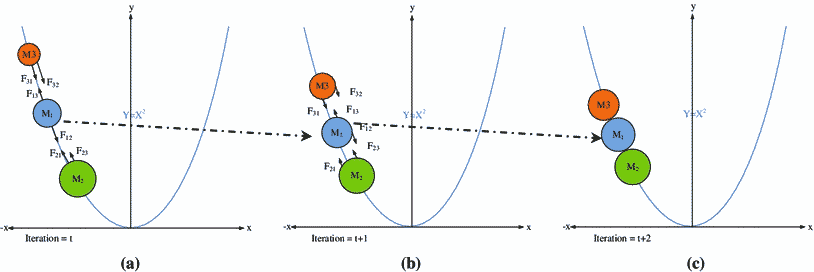
\includegraphics[width=0.8\linewidth]{figures/gsa_neighbourhood_problem.png}
%     \caption{Movement behaviour of neighbourhood near an optimum, Figure 1 from \cite{GGSA}}
%     \label{fig:alg:gsa:neighbourhood-problem}
% \end{figure}

GGSA addresses these two issues by introducing an additional force - a 'global best' solution is kept track of and updated each iteration, and agents are attracted to this 'gbest' solution in the same way they are attracted to the masses of the other agents.
To prevent this from having a significant detrimental effect to early exploration, the gravitational force towards the other agents and the gravitational force towards the gbest solution are weighted separately, with the agent force prioritised during the exploration stage and dropping off as the gbest force is increasingly prioritised during the exploitation stage.

Mirjalili and Lewis \cite{GGSA} did test the performance of GGSA on a wide range of problems, but did not run other optimisation algorithms on these benchmarks aside from GSA.
They tested both algorithms on both a combination of standardised test functions, and a selection of real-world engineering problems, in addition to performing null-hypothesis analysis on the results to determine if their findings were statistically significant.
While all of this testing and analysis suggested that GGSA improved both the exploitation of GSA without compromising its exploitation, the lack of a comparison to benchmark results of other optimisation algorithms makes it difficult to determine if GSA/GGSA should be selected as an optimisation algorithm for a given problem over other optimisation algorithms.
